
% -*- root: These.tex -*-

\subsection{Une lecture pluri-disciplinaire des problématiques liés à la validation}
\label{ssec:triple_lecture}

%Si le modélisateur est au courant des simplifications opérés dans les hypothèses censés représenter ,  la dynamique de construction introduit dans l'activité de construction des modèles une incertitude supplémentaire qui nous oblige à repenser l'activité de validation.


Notre tentative pour pointer quelque une des transformations touchant l'activité modélisatrice dans le giron universitaire entre 1950 et 1970 recoupe bien évidemment la description de vagues d'innovations déjà identifiées par ailleurs, et nous aurons l'ocasion de revenir plusieurs fois sur cette période charnière que sont les années 1970 par la suite. 

L'originalité du travail réside plutôt dans l'identification par une communauté de modélisateurs déjà très hétérogènes d'un ensemble de facteurs limitant le développement et la diffusion de l'activité de modélisation appuyé par l'usage de l'ordinateur. 

Fait quelque peu destabilisant pour un modélisateur cotoyant encore cette expression dans les publications en 2015, le \enquote{problème de la validation} apparait en effet très tôt parmis ces différents facteurs. 

Une question nous vient alors très rapidement à l'esprit, et mérite d'être posé, même si elle on verra par la suite qu'elle est un peu naïve. Comment se fait il que ce problème apparu il a presque 50 ans de façon quasi conjointe avec l'invention et l'adoption de la simulation par différentes communautées de pionniers modélisateurs soit encore aussi présente aujourd'hui, par exemple dans le cadre des publications de communautées fortement inter-disciplinaire comme JASSS ? 

En réalité, s'agit il vraiment du même problème ? Car entre la révolution quantitative partisanne d'une révolution plus globale qui voie les principaux verrou informatique s'effacer ou se déplacer, que faut il encore entendre d'une telle expression ? 

La difficulté d'analyser ce terme à la fois dans ses évolutions temporelles,  et dans sa diversité d'inscription disciplinaire 


\textbf{en interne}

par une communauté hétérogènes de modélisateurs comme dommageable pour la diffusion de cette activité de modélisation sur ordinateur. 


	détour d'une analyse rapide des mutations qu'a subit la modélisation en géographie au détour des années 1970, il est d'ores et déjà visible que la progression informatique n'apparait plus comme la seule contrainte 

Proposer une étude exhaustive de ce terme est délicat

\subsubsection{Les définitions de la validation en V\&V}
\label{sssec:def_generique_validation}

Les termes \foreignquote{english}{Validation \& Verification} ou \textit{V\&V} proviennent à l'origine de l'ingénierie des systèmes, et peuvent être rattachés au concept de \enquote{qualité} tel qu'il est défini par la famille de règles ISO établies par l'organisation mondiale de normalisation.

Décomposable en plusieurs branches cette discipline à part possède une branche dédiée à l'expertise logicielle. De ce fait, il n'existe pas réellement de définition ni de théories ou méthodologies officiellement acceptables, l'acceptation des termes pouvant varier fortement selon les branches d'application.

On trouve toutefois quelques références dans des livres dédiés à la terminologie standard pour la \enquote{gestion de projet} dans un large panel de disciplines, telle que le PMBOK (\textit{A guide to the project Management Body of Knowledge}) \autocite{PMBOK2013}. Résultats d'un travail certifié par des associations ou des organismes étatiques tels que IEEE et ANSI, ce dernier propose une définition générale de ces termes pour l'ingénierie logicielle :

\foreignquote{english}{Verification and validation (V\&V) processes are used to determine whether the development products of a given activity conform to the requirements of that activity and whether the product satisfies its intended use and user needs.}

et revient ensuite plus spécifiquement sur les termes :

\begin{itemize}
\item \textbf{Validation} \foreignquote{english}{The assurance that a product, service, or system meets the needs of the customer and other identified stakeholders. It often involves acceptance and suitability with external customers. Contrast with verification.}
\item \textbf{Verification} \foreignquote{english}{The evaluation of whether or not a product, service, or system complies with a regulation, requirement, specification, or imposed condition. It is often an internal process. Contrast with validation.}
\end{itemize}

Les termes tels qu'ils sont définis sont finalement bien trop généraux pour envisager de les appliquer tels quels dans notre domaine de compétence. Dérivé de la branche de l'\textit{Operational Research (OR)}, les auteurs de la communauté restreinte des \textit{systems analysis or modelling and Simulation (M\&S) } engagent dès les années 1960-70 des efforts pour standardiser ces définitions pour la simulation.

\Anotecontent{first_time_validation}{La citation de Churchman par \textcite{Naylor1966} est tiré de \autocite[165]{Nance2002} : \foreignquote{english}{\foreignquote{english}{X simulates Y} is true if, and only if, (a) X and Y are formal systems, (b) Y is taken to be the real system, (c) X is taken to be an approximation to the real system and (d) the rules of validity in X are non-error-free.} \autocite{Nance2002} }

Parmi les différents auteurs participant de ce mouvement ( Naylor, Finger, Oren, Hermann, Zeigler, Nance, Banks, Gass, Balci, Sargent, etc.), \textcite{Naylor1966} est considéré avec West Churchman (1963) comme un des tout premier à avoir attiré et cristalisé \Anote{first_time_validation} dans de multiples publications l'attention sur cette problématique importante de la V\&V.

Cet économiste formé à l'informatique dans la branche des \foreignquote{english}{management sciences} \autocite{Stricklin1985} est un des premiers en 1967 \autocite{Naylor1967} à publier dans un article nommé \foreignquote{english}{Verification of Computer simulation models} une méthode abordant spécifiquement la question de la crédibilité des connaissances qui peuvent être apportées par un modèle de simulation. Une méthode qu'il va mettre spontanément en tension avec les débats qui agitent la communauté des philosophes à cette même période.

Malgré ces efforts et sa volonté de porter le débat loin dans la communauté inter-disciplinaire (voir les premiers ouvrage collectifs sur l'usage de la simulation dans les \enquote{behavior science} \autocite{Dutton1971, Guetzkow1972} \hl{A verifier}), la démarcation entre les deux termes est encore peu claire \autocites[165]{Nance2002}[3]{Balci1986}. \footnote{\foreignquote{english}{Thomas Naylor, a coauthor of the book cited above, deserves credit for drawing major attention to the validation issue in the 1960s: Is the model actually representing the truthful behavior of the referent system? His work, above and in later publications (Naylor 1971, Naylor and Finger 1967), exerted a major influence in framing validation within different philosophical perspectives. Numerous techniques that can be used were identified or developed. While the issues of both verification and validation were of concern from the early days of simulation, often no clear distinction was made between the two terms.} \autocite[165]{Nance2002}}

\Anotecontent{balci_standard}{\foreignquote{english}{A uniform, standard terminology is yet nonexistent. A recent literature review \autocite{Balci1984} indicated the usage of 16 terms [...] Except some early papers which appearead between 1966 and 1972, model verification and model validation have been most of the time consistently defined reflecting the following differentiation : \textbf{model verification} refers to building the model right; and \textbf{model validation} refers to building the right model. \autocite{Balci1986}}}

Il faudra attendre le début des années 1980 pour qu'un standard émerge, grâce à des financements étatiques \autocite{Balci1986}, mais également du fait des efforts fournis par des auteurs comme Sargent et Balci \autocite{Nance2002}, qui collectent et organisent dans une typologie cohérente l'existant statistique et méthodologique, une activité qu'ils poursuivent encore aujourd'hui \autocite{Balci1998}.\Anote{balci_standard}

Pour \autocite[22]{Oberkampf2010} \foreignquote{english}{A Key milestone in the early work by the OR community was the publication of the first definitions of V\&V by the Society of Computer Simulation (SCS) in 1979 \autocite{Schlesinger1979}}, un des instituts avec la U.S GAO (U.S General Accounting Office) à fournir des spécifications en 1979 \autocite{Balci1986}

\begin{itemize}
\item \textbf{Model Verification} \foreignquote{english}{substantiation that a computerized model represents a conceptual model within specified limit of accuracy.}
\item \textbf{Model Validation} \foreignquote{english}{substantiation that a computerized model within its domain of applicability possesses a satisfactory range of accuracy consistent with the intended application of the model.}
\end{itemize}

\begin{figure}[h]
\begin{sidecaption}[fortoc]{Un des tout premiers schémas issus de la publication de la SCS \autocite{Oberkampf2010,Schlesinger1979}}[fig:S_VV]
  \centering
 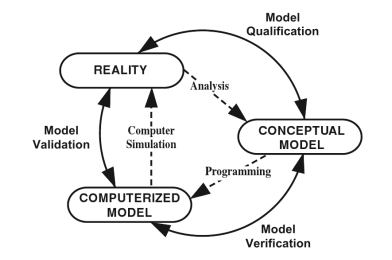
\includegraphics[width=.7\linewidth]{schelinger_schema1979.png}
  \end{sidecaption}
\end{figure}

Même si elles sont plus anciennes et de portée moins générale, ces définitions de la \textit{V\&V} semblent plus pertinentes, car évoquées plus régulièrement par les chercheurs en sciences sociales; les travaux les plus cités étant ceux de \textcite{Kleijnen1995}, ou \textcite{Sargent2010} qui placent leurs travaux dans la continuité de ces définitions. L'avancée de leurs travaux peut être suivie en feuilletant les \textit{Proceedings of the Winter Simulation Conference} où la problématique de la \textit{V\&V} est réévaluée régulièrement au regard des nouvelles connaissances. Ce schéma \ref{fig:S_VV} est devenu un classique repris et régulièrement amendé \autocite{Sargent2010}. Voici la lecture qu'en fournit \autocite{Oberkampf2010}

\foreignquote{english}{The \textbf{conceptual model} comprises all relevant information, modelling assumptions, and mathematical equations that describe the physical process or process of interest. [...] The SCS defined \textbf{qualification} as \enquote{Determination of adequacy of the conceptual model to provide an acceptable level of agreement for the domain of intended application}. The \textbf{computerized model} is an operational computer program that implements a conceptual model using computer programming. Modern terminology typically refers to the computerized model as the computer model or code.}

Ce schéma a la particularité suivante, il \foreignquote{english}{ [...] emphasizes that \textbf{verification} deals with the relationship between the conceptual model and computerized model and that \textbf{validation} deals with the relationship between the computerized model and reality. These relationships are not always recognized in other definitions of V\&V [...]}

\Anotecontent{Kleijnen_def}{\foreignquote{english}{This paper uses the definitions of V \& V given in the classic simulation textbook by Law and Kelton (1991, p.299): \enquote{Verification\textbf{Verification} is determining that a simulation computer program performs as intended, i.e., debugging the computer program .... \textbf{Validation} is concerned with determining whether the conceptual simulation model (as opposed to the computer program) is an accurate representation of the system under study}. Therefore this paper assumes that verification aims at a \enquote{perfect} computer program, in the sense that the computer code has no programming errors left (it may be made more efficient and more user friendly). Validation, however, can not be assumed to result in a perfect model, since the perfect model would be the real system itself (by definition, any model is a simplification of reality). The model should be \enquote{good enough}, which depends on the goal of the model.}}

\Anotecontent{Sargent_def}{\foreignquote{english}{\textbf{Model verification} is often defined as \enquote{ensuring that the computer program of the computerized model and its implementation are correct} and is the definition adopted here. \textbf{Model validation} is usually defined to mean \enquote{substantiation that a computerized model within its domain of applicability possesses a satisfactory range of accuracy consistent with the intended application of the model} \autocite{Schlesinger1979} and is the definition used here. A model sometimes becomes accredited through model accreditation. Model accreditation determines if a model satisfies specified model accreditation criteria according to a specified process. A related topic is model credibility. Model credibility is concerned with developing in (potential) users the confidence they require in order to use a model and in the information derived from that model. A model should be developed for a specific purpose (or application) and its validity determined with respect to that purpose [...]A model is considered valid for a set of experimental conditions if the model’s accuracy is within its acceptable range, which is the amount of accuracy required for the model’s intended purpose.}}

Autrement dit, \foreignquote{english}{The OR community clearly recognized, as it still does today, that V\&V are tools for assessing the accuracy of the conceptual and computerized models.} Un avis partagé par \textcite{Kleijnen1995} \Anote{Kleijnen_def} , \textcite{Balci1998}, et \textcite{Sargent2010} \Anote{Sargent_def} mais également des auteurs de références sur le sujet dans les sciences humaines et sociales \autocite{Amblard2006} \hl{Prend le bout de texte la dessus}.

Seulement, cette forme de relâchement sur la correspondance entre réalité et modèle, et ce positionnement plus relativiste de la validation n'a pas toujours été une évidence; les premières définitions de Naylor par exemple, sont toujours usitées, et continuent si on en croit des auteurs comme \textcite{Kleindorfer1998} à semer le trouble dans certaines disciplines.

\Anotecontent{VV_philout}{ \foreignquote{english}{During the last two decades a workable and constructive approach to the concepts, terminology, and methodology of V\&V has been developped, but it was based on pratical realities in business and government, \textbf{not} the issue of obsolute thruth in the philosophy of nature} \autocite{Oberkampf2010}
\foreignquote{english}{A very old philosophical question is: do humans have accurate knowledge of reality or do they have only flickering images of reality, as Plato stated? In this paper, however, we take the view that managers act as if their knowledge of reality were sufficient. Also see Barlas and Carpenter (1990), Landry and Oral (1993), and Naylor, Balintfy, Burdick and Chu (1966, pp.310-320).} \autocite{Kleijnen1995}
\foreignquote{english}{With the strong interest in verification from the software engineering community, this contrasting but complementary explanation of the term was quite important. The effort to place valida- tion in a cost-risk framework moved the concept from a philosophical explanation in earlier works to a form more useable for simulation practitioners.} \autocite[165-166]{Nance2002}}

Mais en excluant ainsi de son analyse la partie subjective et philosophique de la \enquote{Validation}\Anote{VV_philout} pour se concentrer sur la seule partie opérationnelle, ces méthodologies restent pour le modélisateur une coquille vide décevante, qui demande encore à être incarnée thématiquement. Autrement dit, ces méthodes si elles prennent bien en compte la dimension dynamique et incrémentale nécessaire à la construction d'un modèle de simulation qui tendrait vers une réalité en accord avec la question posée, l'organisation des connaissances nécessaires pour guider ce processus reste à la lecture de ces typologies une opération quelque peu énigmatique pour les modélisateurs géographes. On retombe sur une des critiques soulevées précédemment dans la section \ref{sec:critiques_simulation} sur l'absence constatée dans les publications de méthodologie standard pour la validation qui prendrait en compte les problématiques spécifiques d'une discipline. \footnote{Aujourd'hui des disciplines comme l'écologie proposent des méthodologies plus spécifiques, comme la méthode POM proposé par Grimm sur lequel nous reviendront par la suite \hl{mettre une ref et un appel à la section}}

Une position compréhensible pour ces auteurs oeuvrant pour la standardisation, alors même que ces termes sont toujours d'usages toujours assez variables. Une des conséquences visibles tient dans ces incompréhensions et ces débats terminologiques sans fin \autocite{David2009} que l'on observe parfois en marge des discussions inter-disciplinaires. Cette gamme d'acceptions différentes tient souvent au transfert hasardeux des terminologies entre l'ingénierie des M\&S, la philosophie des sciences, et la thématique d'un chercheur en sciences sociales qui se retrouve en position intermédiaire de ces deux derniers. Un exercice d'équilibriste périlleux, car comme le fait remarquer \textcite{Kleijnen1995} en citant astucieusement une note de bas de page de \textcite{Barlas1990}, en philosophie il est tout à fait possible de voir la signification des deux termes inversée! \hl{Expliquez mieux que verification pourrait se traduire en philosophie pour certains par representation de la vérité, du “reel”, alors que le fait même de modéliser implique qu’on en soit loin}

\subsubsection{La philosophie des sciences}
\label{sssec:philo_sciences}

Il ne s'agit pas de se lancer ici dans un exposé historique des courants et débats s'étant succédés dans cette discipline, mais d'amener de façon illustrative et avec quelques références récentes l'émergence ces 20 dernières années d'une \enquote{épistémologie de la simulation} reprenant (en parasitant parfois le débat comme on l'a cité au dessus) de son point de vue certains débats évoqués chez les praticiens de la simulation; la question de validation étant comme on l'a vu dans le chapitre 1 un sujet de longue date chez les praticiens de la simulation, mais aussi chez les premiers acteurs fondateurs de la V\&V.

\hl{redite : L'objectif n'est donc pas tant de développer une argumentation critique exposant l'ensemble de ces points de vues, car ce n'est pas l'objet de cette thèse, que de tenter de s'insérer (et non de s'enfermer) dans ces réflexions en spécifiant en quoi celle ci diffère, néglige ou font peu écho à nos pratiques et réflexion historique en sciences sociales.}

Le premier obstacle avec laquelle les acteurs supportant cette nouvelle épistémologie doivent cohabités est évidemment la contre-argumentation questionnant cette même necessité d'opérer une nouvelle sous-division épistémologique. Car existe-t-il réellement des spécificité à la connaissance dérivé de l'étude de l'objet simulation, et si oui quelles sont elles réellement ? Autrement dit, existe t il une différence fondamentale entre les questionnements déjà posés dans le cadre d'une épistémologie des modèles et ceux évoqués dans le cadre d'une épistémologie de la simulation ?

\Anotecontent{frilosite_philoScience}{\foreignquote{english}{As computer simulation methods have made their way into novel disciplines, the issue of their trustworthiness for generating new knowledge has often loomed large, especially when they have competed for attention with experiments or analytically tractable modeling methods. The relevant question is always whether or not the results of a particular computer simulation are accurate enough for their intended purpose.[...] Given our long-standing preoccupation with issues of confirmation, it might seem obvious that philosophers of science would have the resources to easily approach these questions.} \autocite{Winsberg2013}}

parmi les auteurs ouvertement favorable à la création d'une nouvelle épistémologie, on citera entre autre les efforts de \autocites{Winsberg2001, Winsberg2009, Winsberg2013} qui pousse dans chacune de ses publications les \enquote{philosophes des sciences} à sortir de la seule étude de la \enquote{théorie de la confirmation} pour aller vers un terrain un peu plus aventureux \Anote{frilosite_philoScience}, celui de l'étude de la crédibilité des explications et des hypothèses dans leur dépendance au contexte.

Il propose de résumer l'originalité d'une telle épistémologie en évoquant l'inférence spécifique que produisent l'étude simultanée de trois point sur la simulation. \foreignquote{english}{ \textcite{Winsberg2001} argued that, unlike the epistemological issues that take center stage in traditional confirmation theory, an adequate EOCS must meet three conditions. 
downward, motley, and autonomous.[...] These three features were meant to be offered as conditions of adequacy; for which any adequate epistemology of simulation must account. Against the background of the growing use of simulation in the sciences, an adequate epistemology for the philosophy of science needs to explain the fact that simulation results and computational models are often taken to be reliable despite these three features. Winsberg (2001) argues that simulation requires a new epistemology precisely because traditional stories in philosophy of science about how knowledge claims get credentialed cannot explain them.}

Cette typologie a soulevé un certain nombre de critiques chez les philosophes des sciences, dont la plus longue et la plus argumenté est surement celle de \textcite{Frigg2009} dont on trouve le résumé des points saillants dans les publications de \textcites{Winsberg2009, Winsberg2013} mais également de bien d'autres auteurs qui se réfèrent à ce débat pour se positionner \textcites{Yanoff2010, Eckhart2010}.

Le deuxième point de débat intéressant réside dans le qualificatif souvent donné à la simulation de \enquote{laboratoire virtuel pour l'expérimentation}. Si les philosophes des sciences ne peuvent que s'incliner face au constat d'une telle banalisation du terme, dont nous avons donné nous même un aperçu de son ancienneté d'usage dans les sciences sociales dans le chapitre 1; il existe quand même chez les philosophes la volonté de mettre à l'épreuve les fondements et les conséquences pour la connaissance extraite d'une telle analogie.

\Anotecontent{HackingCartwright}{\enquote{Nos deux livres ont plus d'un point commun. L'un et l'autre accordent peu d'importance à la vérité des théories et avouent un faible pour certaines entités théoriques. Cartwright soutient que seules les lois phénoménologiques de la physique parviennent à la vérité tandis que, dans la partie B de ce livre, je fais remarquer que la science expérimentale est plus indépendante de la théorie que ce que l'on veut bien généralement admettre. Nous ne partons pas des mêmes postulats anti-théoriques car elle considère les modèles et les approximations alors que c'est surtout l'expérience qui m'intéresse, mais nos conceptions convergent.}\autocite{Hacking1983}}

\Anotecontent{Phan_Varenne_theorie}{\foreignquote{english}{Consequently, in the first neo-positivist epistemology, models were viewed not as autonomous objects, but as theoretically driven derivative instruments. Following the modelistic turn in mathematical logic, the semantic epistemological conception of scientific models persisted to emphasize on theory.} \autocite{Phan2010}}

Un débat d'autant plus actif qu'on assiste depuis ces 20 dernières années à un véritable renouveau des questionnements dans le cadre d'une \enquote{épistémologie de l'expérimentation} jusqu'alors relativement peu considéré par la majorité des philosophes des sciences \Anote{Phan_Varenne_theorie}. \textcites{Phan2008, Phan2010} citent ainsi les contributions importantes d'auteurs comme Fischer(1996), Galison (1987, 1997), Franklin (1986, 1996), Morrisson(1993, 1999), mais également les efforts de Hacking (1983) et Cartwright.

\Anotecontent{def_cartwright}{\enquote{Disons qu'il y a des théories, des modèles et des phénomènes. Il serait normal de penser que les modèles sont doublement des modèles. Ils sont modèles pour les phénomènes et modèles pour la théorie. [...] Le réalisme scientifique est ici tout particulièrement concerné. Cartwright est pour l'essentiel anti-réaliste à propos des théories. Pour cela, elle s'appuie en partie sur les modèles. Elle fait remarquer que non seulement les modèles ne peuvent être déduits de la théorie qui les englobe, mais plus encore que les physiciens utilisent à leur gré divers modèles qui, sans pourtant se recouper, cohabitent tous au sein de la même théorie. Et cependant,ces modèles sont les seules représentations formelles disponibles des lois phénoménologiques que nous tenons pour vraies. Elle affirme que seules ces lois phénoménologiques nous permettent d'avancer. Toutes les modélisations de ces lois ne peuvent être vraies ensemble puisqu'elles ne sont pas compatibles. Et rien ne permet de penser qu'un modèle est supérieur à un autre. Aucun n'est vraiment justifié par la théorie qui le porte. Plus encore, les modèles ont tendance à résister aux changements de théorie, c'est-à-dire que le modèle est conservé même si la théorie s'avère inadéquate. Il y a plus de vérité locale dans les modèles incompatibles que dans les théories, pourtant plus sophistiquées.[...] L'idéal de la science n'est pas l'unité mais dans une abondance et diversité de plus en plus grandes.} \autocite[350]{Hacking1983}}

\Anotecontent{def_hacking}{\enquote{Le \textit{réaliste à propos des entités} affirme que bon nombre d'entités théoriques existent vraiment. L'anti-réaliste s'oppose à ces entités qui ne sont pour lui que fictions, constructions logiques ou éléments d'un processus intellectuel d'appréhension du monde. Un anti-réaliste moins dogmatique dirait que nous n'avons pas, et ne pouvons avoir, de raison de supposer que ces entités ne sont pas des fictions. Peut-être existent-elles,mais le présupposer n'est pas nécessaire à notre compréhension du monde.

Le \textit{réaliste à propos des théories} dit que les théories
sont soit vraies, soit fausses et ce indépendamment de ce que nous percevons : la science, elle au moins, vise à obtenir la vérité et la vérité est le monde tel qu'il est. L'anti-réaliste dit des théories qu'elles sont au mieux
prouvées, adéquates, opératoires, acceptables - quoi-que incroyables, entre autres qualificatifs possibles.} \autocite[59]{Hacking1983}}

On retiendra principalement pour notre argumentaire cette propriété d'indépendance retrouvé de l'expérimentation par rapport à la théorie \Anote{def_cartwright}, dont on peut trouver un très bon manifeste dans les écrits de \textcite{Hacking1983} et Cartwright \Anote{def_hacking}, ces derniers se positionnant comme des antiréalistes des théories, tout en étant des réalistes des entités théoriques. Un point de vue très bien résumé à la fois dans \textcite{Hacking1983} et \textit{Théorie, Réalité, Modèle} de \textcite[226-231]{Varenne2012}

Sur la notion de modèle dans sa relation à l'expérimentation, il semblerait qu'un consensus se dégage chez les philosophes \autocites{Morgan2009, Varenne2013} autour du modèle perçu comme un \enquote{médiateur autonome} articulant théorie, pratiques et données dans un contexte spécifique d'une question et d'un cadre technico-social. \autocite[2]{Phan2010}

Il y a probablement un point intéressant à développer entre cette argument du modèle autonome, et les récents travaux en sciences sociales pour qualifier au travers d'une grille de lecture \autocites{Banos2013a, Sanders2013} le positionnement \autocites{Banos2013, Schmitt2013} et le déplacement des modèles de simulation au travers d'une part de leur construction \autocite{Cottineau2014b}, mais également de leur réutilisation \autocite{Schmitt2014}. Une autre façon de démontrer en quoi cette capacité à cumuler de façon flou différentes fonctions épistémiques donné dans la spécification minimale de Varenne pour la simulation \autocite{Varenne2013} est intéressante dès lors qu'il s'agit de tracer la trajectoire disciplino-temporelle de certains modèles : daisyWorld \autocite{Dutreuil2013}, Schelling \autocite {Bulle2005}, SugarScape, etc.)

\Anotecontent{winsberg_exper_simu_link}{Another unique feature of the epistemology of simulation is the ease with which it can draw inspiration from the epistemology of experiment.}

Les acteurs pronant comme Winsberg une épistémologie de la simulation n'hésite alors pas à débattre pour ce qui est des différents parallèle que l'on peut tracer avec les réflexions de cette communauté. \Anote{winsberg_exper_simu_link}.

Pour ne pas se perdre dans les différents points de vues sur le sujet et bénéficier d'une vue plus large incluant les réflexions des praticiens, on pourra se référer au travail opéré par \textcite{Varenne2001} dans son article \textit{What does a computer simulation prove?}, qui propose une lecture du débat au travers de d'une typologie soulevant trois grandes thèses : I - La simulation est elle un outils commes les autres \textit{A simulation is only a tool} ? II - ou bien l'équivalent fusionnel d'une expérimentation classique (\textit{A simulation is an experiment}) ? III - ou se positionne-t-elle comme médiateur entre la théorie et expérimentation ? (\textit{A computer simulation is an intermediate between theory and experiment})? 

%L'expérimentation mène sa vie propre et entretient diverses relations avec la spéculation, le calcul, la construction de modèles, l'invention et la technologie. Mais alors que le calculateur, le spéculateur et le constructeur e modèles peuvent être anti-réalistes, l'expérimentateur, lui, doit être réaliste. p18 

On trouve donc un grand nombres de travaux, toutes disciplines confondues (les philosophes des sciences ne sont pas les seuls à se poser ce type de question, comme nous verrons par la suite), qui tentent d'établir par le biais de différentes grilles de lecture l'appartenance de ce \enquote{nouveau?} mode d'expérimentation à une des catégories de cette grille. \textit{Pourquoi ? Au delà du jeu d'esprit, quel est l'enjeu motivant une telle comparaison ?}

\Anotecontent{moto_hacking}{Une remarque qui renvoie d'ailleur explicitement à sa lecture du moto d'Hacking \foreignquote{english}{experiments have a life of their own} et à la notion d'autonomie (\textit{autonomous}) de sa synthèse précédemment, qui marque le fait que dans certains cas (impossibilité d'observation, manque de données), la simulation doit faire la preuve des connaissances (\textit{background knowledge}) apportés sur appel de ses propres ressources.}

\Anotecontent{experimental_warranting_belief}{\foreignquote{english}{The central idea of this thread is that experiments are the canonical entities that play a central role in warranting our belief in scientific hypotheses, and that therefore the degree to which we ought to think that simulations can also play a role in warranting such beliefs depends on the extent to which they can be identified as a kind of experiment} \autocite{Winsberg2009}}

Partant du fait que l'expérimentation joue un grand rôle dans l'établissement d'une crédibilité pour les hypothèses avancés, il s'agit de mesurer à quel point la simulation serait susceptible d'apporter les mêmes garanties dès lors qu'on accepte de la voir comme une sorte d'expérimentation.\Anote{experimental_warranting_belief}

On s'appuiera dans la suite de cette argumentation sur la lecture de Winsberg, un philosophe des sciences que l'on estime plutôt partisan de la III thèse dans la classification ci dessus. Ce dernier s'appuie largement sur les travaux d'Hacking, mais aussi Galison pour construire sa réflexion, par exemple en arguant\foreignquote{english}{ [...] that some of the techniques that simulationists use to construct their models get credentialed in much the same way that Hacking says that instruments and experimental procedures and methods do; the credentials develop over an extended period of time and become deeply tradition-bound.} \autocites{Winsberg2003, Winsberg2013} \Anote{moto_hacking}

Winsberg résume ce débat en deux thèses opposés : \foreignquote{english}{Identity Thesis} qui consiste à dire que la simulation est littéralement une expérimentation, et \foreignquote{english}{Epistemology Identity Thesis} qui consiste à penser qu'il existe une dépendance entre les garanties de crédibilité qui pourront être accordé par les résultats de la simulation et leur capacité à être plus ou moins définie en tant qu'expérience. Si la première thèse semble assez bien correspondre au point I de la classification de Varenne, la deuxième semble être une sous-variation du point I.

La plupart des auteurs cités par la suite dans ce débat sont des philosophes des sciences spécialisé en économie (Guala , Morgan, Maki, Simon ) qui rejettent comme Winsberg (plus spécialisé en physique) assez naturellement ces deux thèse \autocite{Winsberg2009}, mais avec des arguments assez différents, qu'il convient d'évoquer pour bien comprendre la complexité de ce débat, assez théorique. 

\Anotecontent{maki_phan}{\foreignquote{english}{For Mäki, abstractions in models are similar to abstractions in experiments as they both can be interpreted as a kind of isolation [...] This analogy between models and experiments is called \enquote{isolative analogy} by Guala (2008). From Mäki’s standpoint, a model can be said to be experimented in its explanatory dimension: the finality of such a model is to explore the explanatory power of some causal mechanism taken in isolation.} \autocite{Phan2008}}

parmi les différents point de vue existant, on citera par exemple le sous-débat de l'\foreignquote{english}{isolative analogy} relaté ici au travers des publications de \textcite{Phan2008, Phan2010} apellant les points de vue de Morgan et Guala contre Maki (2005). Ce dernier voit dans la similitudes entre isolement théorique du modèle comme expérience de pensée et isolement expérimental \Anote{maki_phan} la possibilité de rejoindre une des deux thèses évoqués par Winsberg, établissant d'une façon ou d'une autre que \textit{les modèles sont des expériences, et les expériences des modèles}. Mais ce type d'argument, et on le suppose tout ceux qui se rapportent à l'évocation d'analogies pour justifier d'une équivalence de puissance épistémique se heurterai, comme on va le voir, à une différence fondamentale.

\Anotecontent{guala_phan_winsberg}{Winsberg résume le point de vue de Guala(2002) ainsi \foreignquote{english}{Guala argues that simulation differ fundamentally from experiments in that the object of manipulation in an experiment bears a material similarity to the target of interest, but in a simulation, the similarity between object and target are merely formal.}, mais on peut trouver une version réactualisé en 2008 dans l'article de \textcite[4.2]{Phan2010} \foreignquote{english}{In a simulation, one reproduces the behavior of a certain entity or system by means of a mechanism and/or material that is radically different in kind from that of a simulated entity (...) In this sense, \enquote{models simulate} whereas \enquote{ experimental systems} do not. Theoretical models are conceptual entities, whereas experiments are made of the same \enquote{stuff} as the target entity they are exploring and aiming at understanding}\autocite[14]{Guala2008}}

\textcite{Phan2010} et \textcite{Winsberg2013} cite le point de vue de Guala (2002, 2008), partagé par Morgan(2002, 2005) et se référant aux travaux de Simon (1969). Ceux-ci s'appuient sur une différence de relation qui existe entre système à étudier et système cible dans chacun des deux cas. En effet, dans le cas des expérience, la comparaison s'appuie avant tout sur une similarité matérielle, alors que dans le cas de la simulation la comparaison est limité à une comparaison formelle entre les objets.\Anote{guala_phan_winsberg}

\Anotecontent{Winsberg_critique_morvan}{\foreignquote{english}{Interestingly, while Morgan accepts this argument against the identity thesis, she seems to hold to a version of the epistemological dependency thesis. She argues, in other words, that the difference between experiments and simulations identified by Guala implies that simulations are epistemologically inferior to real experiments - that they have intrinsically less power to warrant belief in hypotheses about the real world.} \autocite[841]{Winsberg2013}}

Morgan(2002, 2005) accepte le point de vue Guala et Simon, mais s'en sert pour réduire indirectement le pouvoir épistémique de la simulation. Un argument bien résumé par \textcite{Phan2008} \enquote{Pour Morgan (2005) modèles et expériences partagent des fonctions de médiateurs et peuvent fonctionner \textit{sur un mode expérimental}, mais les expériences \textit{réelles} offrent un \textit{pouvoir épistémique} d'investigation de la réalité empirique plus fort.} Ce qui fait dire à Winsberg que Morgan serait indirectement plutot partisan de sa deuxième thèse.\Anote{Winsberg_critique_morvan}
\Anotecontent{winsberg_mereformal}{\hl{A compléter avec ce que dit Winsberg2013}}

Pour \textcite{Winsberg2009} le flou des arguments avancé par Morgan et Guala  (\textit{material similarity}, \textit{mere formal similarity}) ne permet pas d'exclure complétement et définitivement la première thèse.\Anote{winsberg_mereformal} Celui-ci se range malgré tout du coté de Guala, et préfère là aussi rejetter cette thèse, mais à la faveur de sa propre argumentation; ce qui lui permet de rejetter à la fois l'argument Morgan pointant l'infériorité épistémique de la simulation, et la deuxième thèse. Il argue que les simulations et l'expérience diffère principalement par la nature du \textit{background knownledge}, c'est à dire protocoles et les connaissances mobilisés.

Des modélisateurs et épistémologues en sciences sociales beaucoup plus proche de nos pratique comme Phan et Varenne trouve un argument convaincant dans ce dernier point, car \foreignquote{english}{Aujourd'hui, comme le souligne Winsberg, la crédibilité des modèles de simulation repose largement sur la \textit{confiance} que nous pouvons avoir dans les compétences des modélisateurs, informaticiens, expérimentateurs et observateurs, ainsi que dans les composants ou plateformes qui supportent les expériences de simulation.} \textcite{Phan2008}

\Anotecontent{gilbert_critique}{\foreignquote{english}{\enquote{[t]he major difference is that while in an experiment, one is controlling the actual object of interest (for example, in a chemistry experiment, the chemicals under investigation), in a simulation one is experimenting with a model rather than the phenomenon itself.} \autocite[14]{Gilbert2005}. But this doesn't seem right. [...] It is false that real experiments always manipulate exactly their targets of interest. In fact, in both real experiments and simulations, there is a complex relationship between what is manipulated in the investigation on the one hand, and the real-world systems that are the targets of the investigation on the other. In cases of both experiment and simulation, therefore, it takes an argument of some substance to establish the ‘external validity’ of the investigation – to establish that what is learned about the system being manipulated is applicable to the system of interest. Mendel, for example, manipulated pea plants, but he was interested in learning about the phenomenon of heritability generally \autocite{Winsberg2013}}}

\Anotecontent{guala_morgan_reality_experiments}{\foreignquote{english}{The identity thesis itself has drawn criticism from Guala (2002) and Morgan(2002). Guala begins by dismissing what he takes to be a poor argument against it. The poor argument goes something like this : simulations are not at all like real experiments because real experiments manipulate the real-world systems that are the very target of the investigation, while simulation merely manipulate \enquote{models} of the target system. What both Guala and Morgan correclty point out is that it is, quite generally speaking, false.}}

Autre sous-débat évoqués par \textcite{Winsberg2013}, on suppose en partie en réponse à sur son article précédent et très similaire \autocite{Winsberg2009}, la critique de l'\textit{identity thesis} comme évoqué par Gilbert et Troitzsch (1999), dont il pense \Anote{gilbert_critique}, en accord avec Guala (2002) \autocite{Winsberg2009} mais également Morgan et Parker \autocite{Winsberg2013} qu'elle est un argument trop faible pour rejeter l'\textit{identity thesis}. \Anote{guala_morgan_reality_experiments} 

Si les arguments de Winsberg semblent convaincant, \textcites{Peschard2010b, Peschard2013} tente dans une analyse critique d'en montrer les biais, et apporte dans son article des objections tout à fait crédible issue de son domaine d'expertise. Pour ne citer qu'un de ces argument, si il existe bien un intermédiaire de mesure issue d'un modèle, comme l'indique Winsberg, il existe également un sous système en prise directe avec la réalité physique de ce monde. En conclusion, elle estime que si il y a bien une certaine forme de similarité entre cibles épistémiques de la simulation et de l'expérience, pour elle ces activités ne peuvent pas être épistémiquement équivalentes, ce qui n'empeche en rien selon elle la coopération fructeuse des deux approches. \hl{Ajouter une footnote avec explication}

\textcite{Winsberg2013} résume le point de vue de \autocite{Peschard2010} ainsi, \textit{Thus, simulation is distinct from experiment, according to her, in that its epistemic target (as opposed to merely its epistemic motivation) is distinct from the object being manipulated.} Autrement dit, même si la motivation menant à l'expérience est bien eloigné (la motivation), l'objet manipulé dans une expérience est bien celui du monde physique, alors que dans le cas de la simulation c'est l'ordinateur. Or autant la motivation peut apprendre de l'objet manipulé dans le monde physique, autant il n'est pas ici dans notre intérêt d'apprendre sur l'ordinateur en tant qu'objet. Dans ce cas là on pointe une différence, mais on peut également appeler selon \textcite{Winsberg2013} et Morrisson (2009) l'argument inverse pointant au contraire une similarité. L'objet expérimenté étant le plus souvent choisi en tenant compte justement de sa capacité de \textit{surrogate} rapport à la question que l'on se pose effectivement, un point commun entre la construction de simulation et d'expérimentation. 

Winsberg conclu en ajoutant que l'expérimentation, contrairement à ce que l'on pourrait penser, n'est pas forcément et immédiatement plus crédible si on ne lui ajoute pas un bagage de connaissance : \textit{Experiments are not automatically more reliable than simulations, despite their differences. [...] It would seem that there are identifiable differences between ordinary experiments and simulations, but there is nothing about these differences that makes one or the other intrinsically more epistemically powerful.}  \autocites{Winsberg2009, Winsberg2013}

\textcite{Varenne2001} avance alors un autre argument intéressant : \foreignquote{english}{Indeed, when you read (Von Neumann 1951), you see that analog models are inferior to digital models because of the accuracy control limitations in the first ones. Following this argument, if you consider a prototype, or a real experiment in natural sciences, is it anything else than an analog model of itself? The test on the prototype is a real experiment. But is it something different and better than the handling of an analog model? So the possibilities to make sophisticated and accurate measures on this model - i.e. to make sophisticated real experiment - rapidly are decreasing, while your knowledge is increasing. These considerations are troublesome because it sounds as if nature was not a good model of itself and had to be replaced and simulated to be properly questioned and tested! It looks as if it was not possible any more to end a paper on simulation by reassuringly using the traditional word: \enquote{Simulation will never replace real experiments”.} }

Ces derniers paragraphes montrent que le débat est loin d'être fixé, et il semblerait là encore que ce soit la définition du contexte d'application qui détermine le mieux la capacité explicative de la simulation, car comme le dit Winsberg \enquote{l'impossibilité d'expérimenter} existe dans bien des disciplines, comme les sciences sociales, mais également la biologie ou la physique, ou les tentatives de reconstitution simulé d'univers ou d'étoiles dans des super calculateur de plus en plus puissant montre qu'il existe un interet explicatif à cette pratique. On pensera notamment aux projets d'expérimentation récents extremement complexe et couteux en physique (laser megajoule de bordeaux, projet ITER pour la fusion).

Et c'est sur ce point que l'argumentation de la plupart des philosophes des sciences est tout à la fois aussi intéressant que problématique. Pour continuer sur Winsberg, celui ci traite de ces problématiques en se positionnant uniquement du point de vue des sciences physiques. Un fait dont il reconnait prudement les conséquences que peuvent avoir l'inclusion d'un contexte différent sur sa synthèse : \foreignquote{english}{Parker (forthcoming) has made the point that the usefulness of these conditions is somewhat compromised by the fact that it is overly focused on simulation in the physical sciences, and other disciplines where simulation is theory-driven and equation-based. This seems correct. In the social and behavioral sciences, and other disciplines where agent-based simulation (see 2.2) are more the norm, and where models are built in the absence of established and quantitative theories, EOCS probably ought to be characterized in other terms.

For instance, some social scientists who use agent-based simulation pursue a methodology in which social phenomena (for example an observed pattern like segregation) are explained, or accounted for, by generating similar looking phenomena in their simulations (Epstein and Axtell 1996; Epstein 1999). But this raises its own sorts of epistemological questions. What exactly has been
accomplished, what kind of knowledge has been acquired, when an observed
social phenomenon is more or less reproduced by an agent-based simulation?
Does this count as an explanation of the phenomenon? A possible explanation?
(see e.g., Grüne-Yanoff 2007).

It is also fair to say, as Parker does (forthcoming), that the conditions outlined above pay insufficient attention to the various and differing purposes for which simulations are used (as discussed in 2.4). [...] Indeed, it is also fair to say that much more work could be done in classifying the kinds of purposes to which computer simulations are put and the constraints those purposes place on the structure of their epistemology.}

Des philosophes des sciences ont donc saisi cette opportunité de critiquer l'approche de Winsberg pour soulever dans des tentatives de typologies parfois intéressantes \autocite{Eckhart2010} les points de divergences que soulève l'utilisation d'une philosophies des sciences naturelle inadapté à la simulation en sciences sociales. Malheureusement, au cours de ces mêmes lectures, on constate que cette critique se retourne vers les modélisateurs et praticiens des sciences sociales, et mène cette fois ci dans une analyse incomplète du contexte historique au mieux à des interprétations erronés (voir le débat animé entre \autocite{Yanoff2008}  \autocites{Elsenbroich2012, Chattoe2011}), et au pire à des approximations et  conseils de mise en oeuvre totalement déplacé \autocite{Eckhart2010} vis à vis de disciplines qui disposent comme on l'a vu d'une véritable histoire autour de l'usage des méthodes computationelles.

Car bien que la recherche des points communs et des différences entre réalité de l'expérimentation physique et virtuelle apparaisse comme un débat intéressant, il faut bien avouer que celui ci ne peut que difficilement s'adapter à la quasi absence d'expérimentation au sens classique dans les sciences sociales. Ainsi, même si la simulation partage certaines des propriétés de l'expérimentation classique, il y a quand même quelque chose de paradoxal à vouloir absolument analyser le rapport de la simulation à l'expérimentation alors même que c'est cette absence qui justement motive son utilisation dans notre discipline, hormis peut etre pour mettre plus en avant cette incapacité à formuler un unique cadre fédérateur par un tel débat. Comme le dit très justement \textcite{Phan2008} {[...] les sciences économiques et sociales sont plus volontiers concernées par l’opposition entre \enquote{le modèle et l’enquête}  (Gérard-Varet et Passeron, 1995) que par celle entre \enquote{l’expérience et le modèle} (Legay, 1997)}

La notion de modèle vue comme médiateur autonome entre théorie et modèle doit elle aussi être repensé pour les sciences humaine, et la géographie; car les théories si elles peuvent exceptionnelement servir à dériver des modèles, celle ci ne peuvent qu'être difficilement rapporté à leur équivalent en science physique \autocite{Pumain1997}.

D'un coté les sciences physiques semble encore viser l'etablissement d'un cadre fédérateur alors qu'il semble que les théories et les modèles en sciences sociales - hormis peut être le cas particulier de l'économie - soit au contraire pourvoyeur de richesse dans leur capacité à apporter un nouvel éclairage sur un phénomène observé. \hl{a préciser peut etre}

A cela il faut ajouter que le modèle en géographie opère dans un cadre épistémique particulier qui n'est pas forcément celui de toute les sciences humaines. Ainsi, bien que les notions et le rapport entre les notions d'observation du \textit{singulier} et du \textit{général} soient théoriquement à la portée de toute disciplines \autocite{Dastes1992}, il semblerait que la géographie trouve un intérét particulier pour la constitution de sa démarche explicative à articuler des éléments de connaissance pris dans les grandes familles explicatives historique, écologique, et spatiale; justifiant ainsi de niveaux d'explication plus ou moins en interaction mobilisant chacun des déterminants de nature différentes. Avec la possibilité d'intégrer à tout moment dans l'explication les résidus qui tiennent d'un dialogue entre méchanismes généraux et singularité historique, écologique ou spatiale. Car quelque soit le registre explicatif choisi il reste dans les deux cas \textit{ [...] une part d'explication relevant de ce que l'on peut qualifier de singularités locales, non prédictibles à partir de mécanismes généraux, mais nécessitant d'appréhender l'histoire spécifique du lieu}. La conséquence étant une diversité de modèles support de l'explanan (l’explication que l’on propose du phénomène auquel on s’intéresse) dont l'évolution sur la forme et le fond n'a eu de cesse d'éclairer l'explanandum sous un jour différent. \autocite{Dastes1992, Sanders2000, Sanders2013} \hl{Mais il y a aussi le multi-échelles.}

\hl{A mieux introduire ici} En 1986, lors d'un débat sur les apports de l'AI en géographie, avec les apports de la branche discrete de la simulation, Couclelis montre que les considération philosophiques abordés jusqu'ici sont en réalité très vite abordés par les géographes \foreignquote{english}{A further insight to emerge from discrete model theory, which has some interesting philo- sophical implications, deserves a few comments. The widespread belief that proposing a model corresponds to the assertion that the real phenomena must have some similar structure is contradicted by the sharp distinction between structure and behavior drawn in discrete model theory. Although structure governs behavior, the converse is not true, so that obtaining a model that reproduces some behavior well does not entitle one to make any inferences about the \enquote{real} structure of the phenomenon represented. In fact, it is doubtful whether we may talk about the structure of real phenomena in other than a metaphorical sense. A real system may be no more than the universe of potentially acquirable data.} \autocite{Couclelis1986}

L'éclairage sur la méthodologie sous-jacente à la construction des modèles, pourtant un élément au coeur du raisonnement dans la discipline géographique depuis la révolution quantitative, a encore moins de chance d'être évoqué dans ces publications philosophiques, au détriment d'une réflexion statique plus axé sur la nature de l'objet simulation, et de sa relation au monde.

Or l'évolution des réflexions touchant l'activité de modélisation se construit il me semble à une échelle de reflexion tout à fait différente, celle contextualisé de pratiques guidés par une activité de résolution de questions spécifique à l'analyse spatiale, dont la mise en oeuvre s'appuie sur une chaine de traitements flexibles utilisant à bon escient et de façon cumulative l'arrivée historique de nouveaux outils et avec eux leur capacité à renouveller les questionnements : les statistiques, les modèles, les simulation.

\Anotecontent{ce qui n'est pas sans nous rapeller les difficultés évoqués dans le chapitre 1 sur l'inadéquation et le danger que représente les modes de transmissions actuels.}

\Anotecontent{remarque_Varenne_2001}{\foreignquote{english}{The second thesis of this article is that none of the three categories of arguments could be applied to contemporary sciences in general, whatever their objects, their methods and the moment of their history we consider. None of these three categories could be considered as the only true one. We cannot have a general point of view on the value of computer simulations, because of the different implications and meanings of mathematics in the different fields of science, and because of the various philosophies of nature at stake. This fact remains true for a given field throughout its own history, because the role of mathematics and the definition of the studied object evolve: You cannot find a unique and stable value that would be given to its simulation uses once for all. Again and hopefully, this thesis illustrates the fact that it does not belong to the historian to decide on the value of computer simulation in a given field but to the scientists themselves. These preliminary reflections prove the importance to investigate the intellectual history of contemporary sciences and not only their sociological construction nor their philosophical general insights.}\autocite{Varenne2001}}

Ces rapides remarques nous éclaire sur la latence qui existe entre la réflexion récentes d'épistémologues comme Winsberg, Grüne-Yanoff et la réalité théorique et pratique en géographie. \textcite{Varenne2001} avait déjà bien cerné dans la synthèse faite en 2001 qu'il n'y avait pas dans sa classification une position meilleure ou plus convaincante qu'une autre, la réponse se trouvant comme pour la notion de modèle avant tout dans l'étude du contexte, et donc de l'histoire des disciplines face à cet objet simulation. \Anote{remarque_Varenne_2001} Cela ne veut pas dire que les débats évoqués précédemment en sont automatiquement invalidés, seulement qu'il faut être probablement plus regardant vis à vis des remarques générales et des conclusions beaucoup trop hative qui peuvent parfois en découler. 

Les travaux croisés de praticiens (Pumain, Sanders, Banos), d'épistémologues ou historien des sciences propre à la géographie (Orain, Besse, Robic, Cuyala) ou s'en approchant (Varenne, Phan) permettent d'une part d'apposer un premier filtre sur ces réflexions génériques pour s'y référer prudemment, et d'autre part d'innover en questionnant nos démarches dans ce qu'elles ont d'originales, cette fois ci appuyé sur une lecture des pratiques certe pas toujours parfaite mais pouvant au moins être qualifié de \textit{bottom-up} 

%\hl{Un travail conséquent à la croisée de différentes approches, les travaux d'historiens et épistémologues des sciences somme Orain, Besse, Cuyala, et la lecture plus spécifique de l'évolution des méthodes numériques puis computationelles et de leur apports d'un point de vue pratique et théorique dont on trouve source à la fois dans les nombreux travaux des praticiens, mais également dans des travaux de plus long cours comme celui qu'est en train de réaliser Varenne dans son HDR.  == REDITE}

%\hl{ont su voir rapidement l'intérét de développer plus en avant les spécificités attachés à la simulation en science sociale, déjà riche de réflexion sur les apports successifs et cumulatifs de techniques de simulations \autocites{Banos2013, Varenne2008}, en s'intégrant au débat d'une communauté inter-disciplinaire structuré autour de la modélisation agent, qui émerge dans les sciences sociales au début des années 1990. Ce débat par contre ne fait semble-t-il que commencer dans le courant plus \textit{mainstream} des philosophe des sciences.}

%tel que celle des géographes pratiquant la simulation depuis les années 1950, tels que celle qui a émergé autour de la modélisation agent dans les années 1990. 

%Ainsi comme on a pu le voir dans le chapitre 1, le terme laboratoire virtuel pour l'expérimentation apparait très tot dans les sciences sociales, et des auteurs ont pour l'époque déjà donnés de très bonne raisons pour l'emploi de ce terme; les aspects dynamiques de la simulation en faisait partie.

\subsubsection{La Validation vue par une communauté de modélisateurs centré sur la modélisation agent}
\label{sssec:communautes_jasss}

Depuis le début des années 1990 et la diffusion progressive du méta-formalisme agent \autocite{Treuil2008} dans les sciences humaines et sociales, les modélisateurs géographes peuvent, en plus des pratiques internes à la géographie, se tourner vers les discussions opérés dans une communauté d'acteurs internationaux et inter-disciplinaire. On trouvera sur ce sujet une tentative d'exploration des fondement historiques de ce mouvement dans l'annexe \hl{ref annexe}. Sorti des ouvrages fondateurs, c'est principalement autour du \textit{Journal of Artificial Societies and Social Simulation} (JASSS) fondé en 1998 que gravitent la plupart des discutants pertinents sur la problématique de la Validation. 

Cette étape de validation, l'écueil le plus important surement, est pourtant souvent évoqué comme une étape cruciale dans bon nombres de guides méthodologiques pour \enquote{la bonne construction des modèles}, qu'il soit ancien \autocite[195]{Beshers1965} \autocite{Naylor1966, Naylor1967}, récent \autocite{Amblard2006, Gilbert2008}.

En prenant les écrits de \textcite[301]{Doran1975}, qui fait quasiment figure de co-créateur du mouvement de part son introduction des DAI à Gilbert \autocite{Gilbert1985} (voir également l'annexe déjà cité), on retrouve une filiation directe entre ces écrits de 1975 et 2000 sur cette question, une preuve qui vient s'ajouter à celle déjà évoqué dans le chapitre 1 pour justifier de l'enracinnement de cette problématique dans l'histoire de la simulation.

Ainsi on peut dire que \textcite[300-301]{Doran1975} dans \textit{Mathematical Models and Computer Simulations} est déjà au courant des travaux sur la question dans les sciences sociales, car il cite \autocite{Guetzkow1972}, et reprend à son compte un protocole de construction de modèle dont la description n'a finalement que peu bougé ces dernières années \foreignquote{english}{Any serious simulation study involves major effort at a number of stages : advanced planning; collection and organisation of suitable data; detailed specification of simulation; writing and initial \enquote{debugging} of the computer program; preliminary testing and validation of the program; it's use in the sequence of experiments designed to achieved specified objectives; and finally the study and interpretation of the results obtained. It is easy to underestimate the magnitude of the total effort required.It is all the more important to have a clear idea of what the simulation study is intended to achieve; either a broad investigation of the behaviour of simuland or, more likely, a determined attempt to examine the behaviour of certain variables of interest (cost? death rate? output? public approval?) and to discover to what extent they can be controlled.} 

Si la validation est décrite dans des termes classiques comme une comparaison avec les données, \textcite[301]{Doran1975} soulève par la suite quelles difficultés de l'expérimentation pouvant en définitive grever cette précédente tâche. Car comment valider corectement une simulation compte tenu de tout ces problèmes posés par l'expérimentation ? \enquote{In any simulation, \textit{validation} is a matter of great importance. How can it be ensured that the model is indeed a reliable guide to reality ? [...] Once simulation has been validated it can be put to useful work. At this point a major problem appears. [...] any stochastic simulation must be run many times, and effectively one is sampling the behaviour of the variable of interest. This makes for much book keeping and for many complications.[...] Simulations poses two unexpected experimental problems. First, the number of variables and parameters in the simulation is liable to be very large, [...] Second, it may prove disconcertingly difficult to comprehend what is going on within the simulation, just as it is often difficult to comprehend a complex part of the real outside world. [...] These problems are of more than purely technical interest. They arise from the use of tool of sufficient complexity that it's details can extend human comprehension to the limit.}

En 2000, même si les termes se sont raffinés, et que de nouveau problèmes semblent avoir fait leur apparitions du fait des spécificités de l'outil (aspect cognitif par exemple), le lecteur n'est pas dépaysé sur le fond par la description que fait \textcite{Doran2000} des \foreignquote{english}{Hard problems in the use of agent-based modelling} : \foreignquote{english}{Skills and Time requierement, Which type of Model? , What level of Abstraction ?, Searching a massive parameter space ? The problem of validation ?}

Si on observe bien une constance dans le développement des guides méthodologiques pour la construction de modèles de simulation \footnote{Rajouter comparaison entre deux suites de points}, l'étape ayant attrait à la validation ne reste que très rarement développé ou mis en oeuvre dans des exemples concrets \Anote{grimqualite}. Un exemple encore récent est la publication dans la revue JASSS (dont on rapelle qu'elle a été initié par Gilbert) à la critique cinglante de \autocite{Manzo2007a} vis à vis du guide méthologique établit récemment par \autocite{Gilbert2008}, très concis sur ces questions (7 pages au format A5). Or, si même les auteurs aussi cités et reconnus que Gilbert, qui ont la chance de publier pour la première fois cette méthode dans une collection aussi reconnu (\textit{Sage Quantitative Applications in the Social Sciences}), ne donne pas l'exemple, que doit on attendre des plus jeunes recrues s'essayant à cette technique ?

\hl{Transition}

Toutefois là ou naïvement, avec les évolutions de l'informatique, on aurait pu s'attendre à voir émerger dans les publications des applications concretes permettant d'aborder, même de façon incomplète, cette problématique, ce n'est pourtant pas du tout ce que l'on constate de façon générale.

Dans l'étude mené par \textcite{Heath2009} entre 1998 et 2008 sur 279 publications, l'auteur considère que seul 35 \% des modèles sont validés conceptuellement et informatiquement, même si une amélioration est à noter entre 2005 et 2008, ou ce chiffre monte à 43\% environ. Toutefois, si dans l'ensemble des modèles agents récupérés, on ne garde que les modèles agents classés en science sociale, ce chiffre chute fortement, avec 28\% de modèle validés, et quasiment 37\% de modèle qui n'aborde même pas ce problème \Anote{survey_heath}.

Si on regarde plus du coté des techniques, comme par exemple les analyse de sensibilités, cité régulièrement pour leur utilité dans la \enquote{validation interne} des modèles \autocite{Amblard2006}, le résultat n'est guère plus encourageant. Du moins si on en croit l'étude de \textcite{Thiele2014} entre 2009-2010 \Anote{survey_thiele}, mais également celle plus restreinte de \textcite{Cottineau2015} sur le volume JASSS de Mars 2014 \Anote{survey_cottineau}.

Finalement, sans même faire intervenir les critiques issue de débats plus épistémologiques (comme ceux que l'on a vu précédemment), cette seule insuffisance dans l'utilisation des moyens existants pour évaluer nos modèles suffit largement à prolonger un cercle vicieux où l'absence d'évaluation nourrit une perpétuelle remise en question de cet outil et de sa scientificité \Anote{serpent_mer}. Cette seule connaissances des dynamiques à l'oeuvre dans les modèles ne fait pas tout, mais elle offre déjà une base de discussion marqué par l'honneteté de cette démarche.

A l'image de certain auteurs, on pourra reprocher l'absence d'un protocole plus standard encadrant cette problématique. 

Cette discussion questionne aussi l'absence d'un protocole, d'un standard pour l'évaluation des modèles. %est cité comme un des nombreux écueils avec lequel se bat toujours la discipline, comme en témoigne les discussions réccurentes de nombreux auteurs sur un sujet dont la complexité touche à une dimension technique, que méthodologique ou philosophique. 

Autant d'auteurs \autocite{Richiardi2006} \autocite[198]{Fagiolo2007} \autocite{Moss2008} \autocite{Windrum2007} \autocite{Barlas1996} \autocite{Amblard2003} \autocite{OSullivan2004} \autocite{Doran2000} \autocite{Crooks2012} \autocite{Rouchier2013} dont il faudra par la suite développer les discussions.  


validation des modèles de simulation agents, on se rend compte qu'un certain nombre de problématiques persistent et limitent toujours la diffusion des modèles en dehors du cercle bienveillant de l'inter-disciplinarité \autocite{Richiardi2006}. Ce problème, loin d'être un isolat touchant uniquement les sciences humaines et sociales, existe également dans d'autres disciplines, comme en écologie, où même lorsque les modèles sont publiés, l'absence de protocole pour répliquer, évaluer le modèle est courant \autocite{Grimm1999}. \hl {ref à vérifier}

Un problème qui met un peu plus en danger des communautés de chercheurs dont on sais déjà leur isolement dans certain pays : archéologie, sociologie \autocite{Manzo2007}, et économie \autocites{Lehtinen2007, Richiardi2006} pour n'en citer que quelqu'un. 

cette critique récurrente de l'outil sur le plan de la scientificité, une faiblesse qui constitue toujours un danger pour la pérénité des pratiques inter-disciplinaire autour de la simulation agents \autocite[220]{Squazzoni2010}, a tel point que la communauté se dote de guides de survie pour se protéger des sceptiques. \autocite{Waldherr2013} Est ce là le seul fait d'une mauvaise communication autour de notre discipline comme le laisserait penser la lecture de ces travaux ? 


A : Les approches appliqués les plus sérieuse nous paraissent celle de Grimm, et celle de Behavior search, elles seront commenté en conclusion.

= Article de référence est clairement Amblard 2006

L'article de référence pour la validation de modèle agent en géographie est clairement celui d'Amblard2006, dans le livre dédié à l'agent. Celui-ci ne comportement pas malheureusement de volet applicatif.

= Les géographes interviennent dans cette communautée, exprime forme de détachement

A vouloir mettre en évidence un protocole de validation générique axé autour du seul modèle de simulation, on applanit sans le vouloir une démarche de construction des connaissances mobilisant un ensemble de modèle et de méthode. Il est important de rapeller sans cesse le poids de cet héritage disciplinaire à l'interface de questionnement plus génériques, comme le font régulièrement dans notre discipline Hélène Mathian, Léna Sanders, et plus récemment Cottineau2014b.

Les géographes modélisateurs, même si ils interviennent également au contact de cette communauté, continuent pour certains à développer une approche ou le SMA n'est qu'un outil parmis d'autres hérités d'une longue histoire de la géographie avec la simulation. La question de la validation s'inscrit dans une démarche beaucoup plus globale ou interviennent des multiplicité de modèles et de méthodes.

= Geographes \textbf{centré sur la démarche} et non sur l'outil

Pour raccrocher cette remarque avec les dernières analyses portant sur l'usage des techniques de simulation en géographie, les observateurs (Varenne) tout autant que les acteurs \autocite{Sanders2013}\Anote{sanders_couplage_spirale} de ces pratiques tendent à mettre en avant une tendance croissante à la pluri-formalisation croissante des modèles agents, preuve que cette multiplicité des formalismes et des techniques est de plus en plus considérée comme une richesse dans l'approche de systèmes complexes.

Dans son analyse sur la place de l'explication en analyse spatiale, \textcite{Sanders2000} voit plus dans le rapport de l'outil à la démarche adoptée (exploratoire ou hypothético-deductif) une question d'interprétation, ce qui contextualise encore un peu plus la place de l'outil \enquote{Ce sont en effet la manière dont l'outil est inséré dans une chaîne de réflexion et de traitement et l'interprétation des informations figurant en entrée et en sortie qui permettent de donner le statut descriptif ou explicatif d'une démarche.} Avant de conclure un peu plus loin à la fin de son analyse \enquote{[...]il n'y a pas de relation simple et fixe, ni entre les niveaux d'observation et la nature des explications, ni entre les outils de l'analyse spatiale et l'explication. La variété des approches permet de diversifier les éclairages sur les phénomènes que l'on cherche à expliquer. Nos démarches en analyse spatiale consistent ainsi davantage à \enquote{éclairer} qu'à \enquote{démontrer} et identifier des jeux de causalités bien stricts.}

Pour Maryvonne le Berre encore, \enquote{Il n’y a donc pas d’adaptation de la géographie à la technique mais recherche d’une technique adaptée à chaque objet d’étude géographique}. \textcite{Sanders2013} expose une idée assez similaire de pré-existance des concepts sur l'outils, car pour elle \enquote{La comparaison entre famille de modèles montre qu'il existe des décalages temporels entre la construction conceptuelle d'un champ et la mise au point d'outils appropriés pour la tester. Dans une certaine mesure on peut avancer que les outils \enquote{ont rattrapé} les concepts dans ce champ de recherche.}

= Reste qu'il faut quand meme un support à ce developpement


\subsubsection{synthèse}

% Faire la synthèse des trois approches, notamment en redescendant la partie déjà ecrite à la fin de la partie philo, c'est mieux de noter la spécificité de la géographie pour justifier le fait d'une introspection dans les habitudes de construction en géographie.

Si la communauté \textit{Models\&Simulations} propose aujourd'hui un cadre d'analyse cohérent avec la dynamique attendue chez les géographes pour la construction des modèles, il lui manque toutefois une incarnation géographique qu'il va falloir extraire de nos propres exigences de construction.

Pour comprendre comment la notion de validation se construit en marge de ces deux discours, il faut revenir sur ce qui fait sens dans l'explication pour les géographes. En repartant des transformations que subit la géographie quantitative dans les années 1970 au contact du paradigme systémique, prise dans une nouvelle réflexion des objets géographiques , dont la percolation chez les géographes s'observe dans la nouveauté le champs lexical, les méthodes, mais également les techniques.

Au delà des outils il y a un fond commun, à la construction de modèle en géographie, et qui n'est que très rarement traité dans ces lectures, celui de la mise en œuvre de la construction. Nous verrons qu'il y a des raisons à cela, la dépendance au contexte en est une, et cette activité hautement flexible, bien qu'influencé par la qualité du substrat technique, pose dans la mobilisation des hypothèses des questions génériques à ce dernier : l'hypothèse que j'ai choisi apporte elle un éclairage sur la question posé qui guide la construction du modèle ?

- Oui, et je peux le prouver 

- Non, mais cela ne prouve pas que cette hypothèse n'est en soit pas valable 

Il ya une forme de permanence dans les questions posés par la construction d'un modèle ou d'un modèle de simulation qui apelle à la construction d'une vision de la validation plus appliqué en géographie => ce qui veut dire qu'il lui faudra un support, et cela viendra par la suite

\hl{--------------- Pas fini, tu peux sauter à la partie d'après :) ------}

